\documentclass{beamer}

\usepackage{beamerthemeCVC}

\usepackage{graphicx}

\setbeamertemplate{caption}[numbered]

\usepackage{xmpmulti}


\usepackage{changepage}
% https://tex.stackexchange.com/questions/160825/modifying-margins-for-one-slide


%% PRESENTATION CONFIGURATION PARAMETERS %%%%%%%%%%%%%%%%%%%%%%%%%%%%%%%%%%%%%%%
%  \titlebackgroundfile{images/template_title}
%  \framebackgroundfile{images/template_frame_v05}


%\definecolor{vermell}{HTML}{8C2423}
\definecolor{vermell}{HTML}{000066}
\definecolor{gris}{HTML}{4C4C4C}

% http://latexcolor.com/
\definecolor{anti-flashwhite}{rgb}{0.95, 0.95, 0.96}
\definecolor{palesilver}{rgb}{0.79, 0.75, 0.73}



\usefonttheme[onlymath]{serif}


%Font
% \usefonttheme{professionalfonts}
% \usepackage[utf8]{inputenc}
% \usefonttheme{default}


% \usefonttheme[onlymath]{serif}
% % http://tex.stackexchange.com/questions/34265/how-to-get-beamer-math-to-look-like-article-math



% http://tex.stackexchange.com/questions/183052/what-are-all-the-possible-first-arguments-to-setbeamerfont/183053#183053

\setbeamercolor{title in head/foot}{fg=vermell}


\setbeamercolor{author in head/foot}{fg=palesilver}
%
\setbeamercolor{framenumber in head/foot}{fg=vermell}



\setbeamercolor{section in head/foot}{fg=vermell}
\setbeamercolor{normal text}{fg=gris}
%\setbeamercolor{frametitle}{fg=vermell}
\setbeamercolor{frametitle}{fg=blue!20!black}

\setbeamerfont{block title}{size={}}
\setbeamerfont{author}{size=\footnotesize}
\setbeamerfont{date}{size=\footnotesize}

\setbeamerfont{footline}{size=\fontsize{3}{11}\selectfont}


\setbeamertemplate{itemize item}[circle]
\setbeamertemplate{itemize subitem}[circle]
\setbeamertemplate{itemize subsubitem}[circle]
\setbeamertemplate{itemize subsubsubitem}[circle]
\setbeamercolor{itemize item}{fg=vermell}
\setbeamercolor{itemize subitem}{fg=vermell}
\setbeamercolor{itemize subsubitem}{fg=vermell}
\setbeamercolor{itemize subsubsubitem}{fg=vermell}
\setbeamercolor{enumerate item}{fg=vermell}
\setbeamercolor{enumerate subitem}{fg=vermell}
\setbeamercolor{enumerate subsubitem}{fg=vermell}
\setbeamercolor{enumerate subsubsubitem}{fg=vermell}
\setbeamercolor{alerted text}{fg=vermell}
\setbeamerfont{alerted text}{series=\bfseries}
% This command makes that acrobat reader doesn't changes the colors of the slide
% when there are figures with transparencies.
\pdfpageattr {/Group << /S /Transparency /I true /CS /DeviceRGB>>}



%\setbeamerfont{bibliography entry author}{series=\bfseries}
% \setbeamerfont{bibliography entry title}{series=\bfseries}
% \setbeamerfont{bibliography item}{series=\bfseries}

\setbeamerfont{bibliography item}{size=\scriptsize}
\setbeamerfont{bibliography entry author}{size=\scriptsize}
\setbeamerfont{bibliography entry title}{size=\scriptsize}
\setbeamerfont{bibliography entry location}{size=\scriptsize}
\setbeamerfont{bibliography entry note}{size=\scriptsize}

% \usepackage{hyperref}
% \hypersetup{colorlinks=true, linkcolor=blue}
% \renewcommand*{\bibfont}{\scriptsize}

\graphicspath{{images/}}



%     \setbeamerfont{author}{size=\scriptsize,series=\bfseries,parent=structure}



%%%%%%%%%%%%%%%%%%%%%%%%%%%%%%%%%%%%%%%%%%%%%%%%%%%%%%%%%%%%%%%%%%%%%%%%%%%%%%%%

%      + Short title.               + Title which appears in the cover.
%      v                            v
%\title[Beamer presentation example]{Nonlinear Dynamics Approach to Human Activity Recognition Using Inertial Sensors}
\vspace{5mm}
% \title[Analysis of the Movement Variability in Dance Activities Using Wearable Sensors]
% {Analysis of the Movement Variability in Dance Activities Using Wearable Sensors}
\title[]
{Towards the Analysis of Movement Variability in Human-Humanoid Interaction}
%       + Short author names which appear in the slides.
%       v
\author[Miguel P. Xochicale]
{   % Author names which appear in the cover page.
    %Perez-Xochicale Miguel Angel
    Miguel P. Xochicale\inst{1}, Chris Baber\inst{1} and Mourad Oussalah\inst{2}
}
%          + Short affiliation which appears in the slides.
%          v
\institute[CVC-IIIA]
{   % Affiliation information which appears in the cover page.

      \vspace{5mm}
    \begin{tabular}{c}
    \inst{1} School of Engineering, University of Birmingham, U.K. \\
    \inst{2} Center for Ubiquitous Computing, University of Oulu, Finland
    \end{tabular}
}
%     + Short acronym of the conference or date of the presentation.
%     v
\date[DEMO-2013]
{   % Conference name which appears in the cover page.
      \vspace{5mm}
     HCI Seminars \\
     School of Computer Science, University of Birmingham, UK \\
     26 April 2017
}


% \
% \AtBeginSection[]{
%   \begin{frame}
%   \vfill
%   \centering
%   \begin{beamercolorbox}[sep=8pt,center,shadow=true,rounded=true]{title}
%     \usebeamerfont{title}\insertsectionhead\par%
%   \end{beamercolorbox}
%   \vfill
%   \end{frame}
% }



\newif\iflattersubsect

\AtBeginSection[] {
    \begin{frame}<beamer>
    \frametitle{Outline} %
    \tableofcontents[currentsection]
    \end{frame}
    \lattersubsectfalse
}

\AtBeginSubsection[] {
    \iflattersubsect
    \begin{frame}<beamer>
    \frametitle{Outline} %
    \tableofcontents[currentsubsection]
    \end{frame}
    \fi
    \lattersubsecttrue
}




\begin{document}

\frame{\titlepage}% Creates the cover page.





\begin{frame}
\frametitle{Outline}
\tableofcontents
\end{frame}




%+++++++++++++++++++++++++++++++++++++++++++++++++++
%+++++++++++++++++++++++++++++++++++++++++++++++++++
\section{I. Introduction -- Movement Variablity}

% \frame{\tableofcontents[currentsection]}
% \frame{\tableofcontents[currentsection, currentsubsection]} %new code



  % %+++++++++++++++++++++++++++++++++++++++++++++++++++
\begin{frame}
  \frametitle{Movement Variability is not NOISE}

\vspace{-1cm}
\begin{figure}
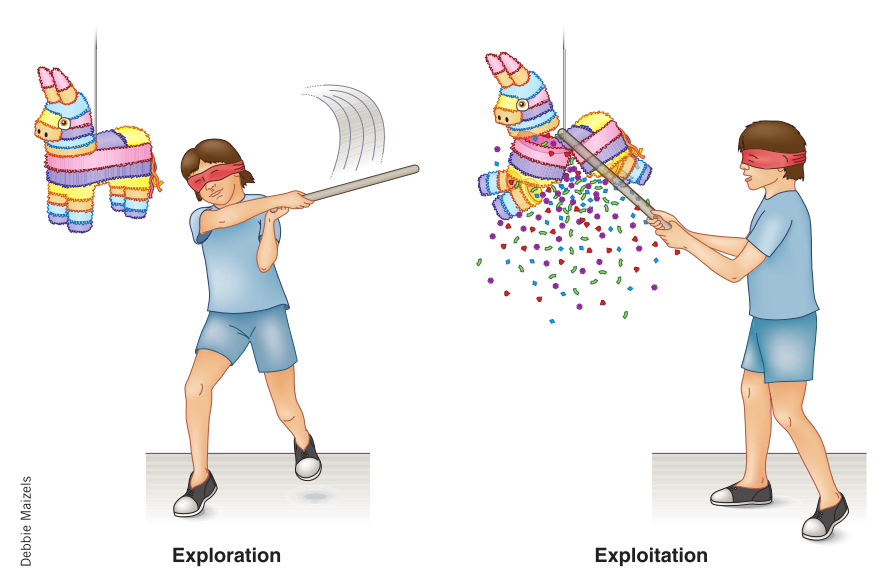
\includegraphics[width=0.9\textwidth]{herzfelt2014_fig1}
\centering
\caption{Find the pi\~nata \textcolor{red}{\textbf{  \cite{Herzfeld2014}   }}.}
 \end{figure}

% \vspace{-5mm}
%   ... better exploration (characterized by movement variability) in the task-specific
%   dimension can contribute to a faster learning rate (exploitation) .

\end{frame}




%%+++++++++++++++++++++++++++++++++++++++++++++++++++
\begin{frame}
\frametitle{Movement Variability}

Movement Variability is an inherent feature that occurs not only within individual
but also between individual systems of movement  \textcolor{red}{\textbf{ \cite{newell1993variability}   }}.

\end{frame}




%%+++++++++++++++++++++++++++++++++++++++++++++++++++
\begin{frame}
\frametitle{How to measure Movement Variability?}


According to \textcolor{red}{\textbf{  \cite{Preatoni2013}   }},
some nonlinear dynamics tools (dynamic invariants)
can be used to explore the nature of movement variability
and its relationship with skills development are:
\begin{itemize}
    \item \textbf{Reconstructed State Space (RSS)},
    \item Lyapunov Exponent.
\end{itemize}


\end{frame}













%+++++++++++++++++++++++++++++++++++++++++++++++++++
%+++++++++++++++++++++++++++++++++++++++++++++++++++
\section{II. Methods --  Reconstructed State Space (RSS)}

% \frame{\tableofcontents[currentsection]}
% \frame{\tableofcontents[currentsection, currentsubsection]} %new code


%  \subsection{Activity Recognition Chain}


%+++++++++++++++++++++++++++++++++++++++++++++++++++
\begin{frame}
\frametitle{Reconstructe State Space (RSS)}
\vspace{-0.7cm}


\begin{figure}[!htb]
\centering
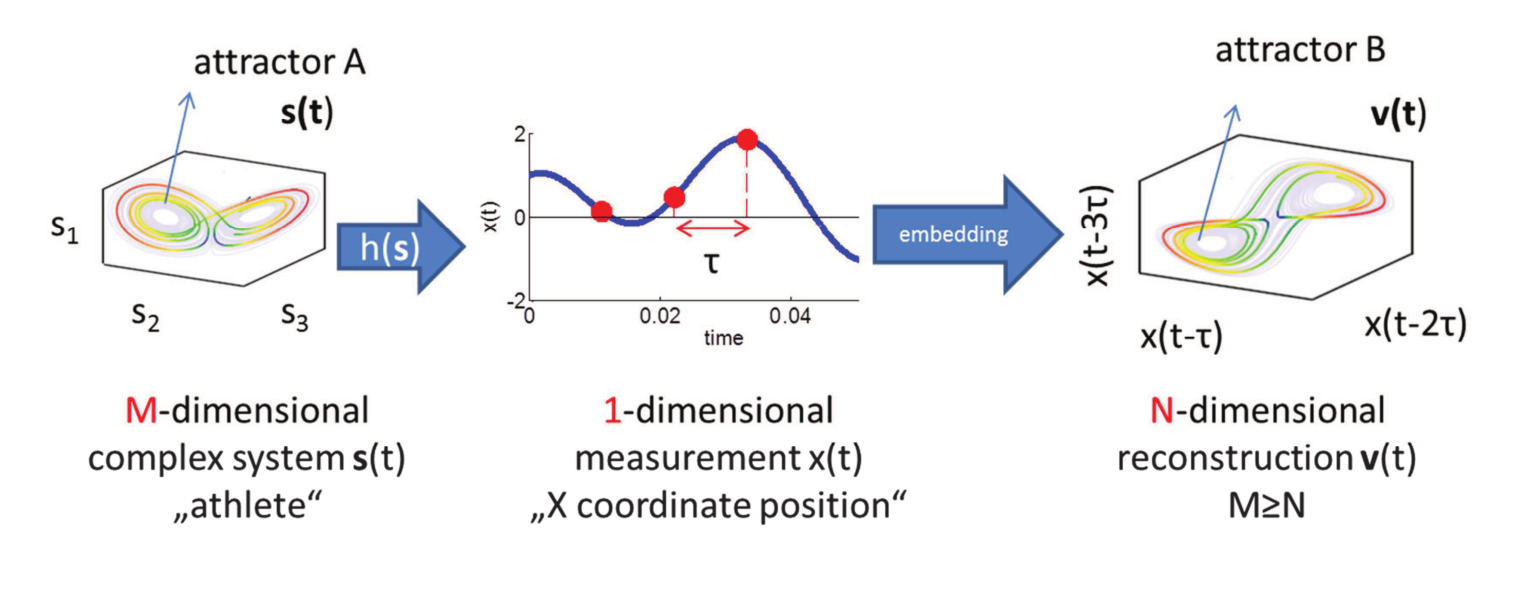
\includegraphics[width=0.95\textwidth]{Quintana-Duque2012_Fig1}
\caption[PA]{Reconstruction of a multidimensional attractor
 \textcolor{red}{\textbf{ \cite{Quintana-Duque2012} }}.
}
\label{fig:sn}
\end{figure}

\end{frame}
%---------------------------------------------------



\subsection{A. RSS in Human-Activity Recognition (HAR) }


% \frame{\tableofcontents[currentsection, currentsubsection]} %new code

%+++++++++++++++++++++++++++++++++++++++++++++++++++
\begin{frame}
\frametitle{RSS in HAR}
\vspace{-0.7cm}


\begin{figure}[!htb]
\centering
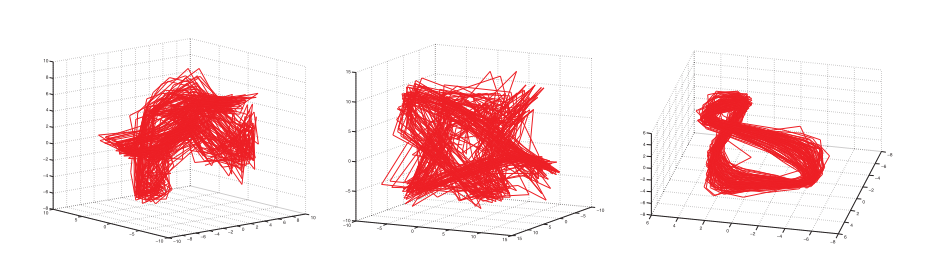
\includegraphics[width=1.05\textwidth]{frank_2012}
\caption[PA]{3D Reconstructed State Spaces ($m=3$, $\tau=4$) for walking (left), running (middle), and cycling (right).
 \textcolor{red}{\textbf{ \cite{Frank2010,Frank2012} }}.
}
\label{fig:sn}
\end{figure}

\end{frame}
%---------------------------------------------------




%+++++++++++++++++++++++++++++++++++++++++++++++++++
\begin{frame}
\frametitle{RSS in HAR}
\vspace{-0.7cm}

\begin{figure}[!htb]
\centering
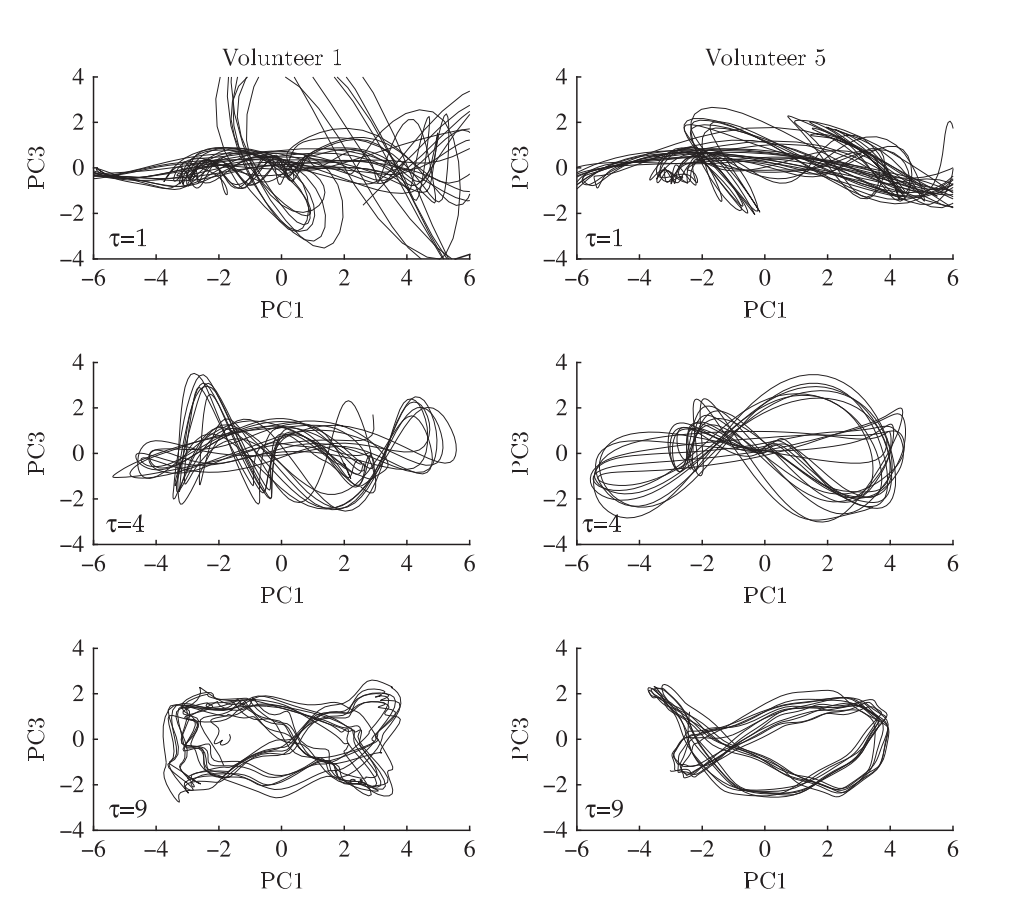
\includegraphics[width=0.625\textwidth]{sama_2013}
\caption[PA]{2D Reconstructed State Spaces for gait patterns of two persons ($m=20$ for $\tau=1$, $\tau=4$ and $\tau=9$, respectively).
 \textcolor{red}{\textbf{ \cite{Sama2013} }}.
}
\label{fig:sn}
\end{figure}



\end{frame}
%---------------------------------------------------






%+++++++++++++++++++++++++++++++++++++++++++++++++++
\begin{frame}
\frametitle{How to build a ReconstructedStateSpace}


For a given discrete time-series $x(n) = [x(1) , x(2), \dots, x(N)]$,
a reconstructed state space can be created by
\begin{eqnarray*}
\overline{x}(n) = [ x(n), x(n - \tau), x(n-2\tau), \dots , x (n-(m-1)\tau) ]
\end{eqnarray*}
which creates a concatenated column-wise matrix of the time-delay versions of the original signal:
\begin{equation}
  \resizebox{\textwidth}{!}{$\displaystyle
  \mathbf{X}
    = \begin{pmatrix} \nonumber
      x(1) & x(1 - \tau) & x(1-2\tau) & \dots & x (1-(m-1)\tau) \\
      x(2) & x(2 - \tau) & x(2-2\tau) & \dots & x (2-(m-1)\tau) \\
      \vdots &  &  & \ddots & \vdots \\
      x(N) & x(N - \tau) & x(N-2\tau) & \dots & x (N-(m-1)\tau) \\
      \end{pmatrix}
     $}
\end{equation}



where $m$ is the \textbf{ embedding dimension}  and  $\tau$ is the \textbf{ embedding delay}
\textcolor{red}{\textbf{  \cite{Takens1981} }}.


\end{frame}
%---------------------------------------------------




%+++++++++++++++++++++++++++++++++++++++++++++++++++
\begin{frame}
\frametitle{Takens' Theorem}

The Takens' Theorem states that for a large enough $m$ is possible to unfold the attractor
and $\tau > 0$ is chosen to maximize the information content of $x(n)$.

\vspace{5mm}

False Nearest Neighborhood and Mutual Information algorithms are used to compute
the optimal value of $m$ and $\tau$. However, as pointed out by  \textcolor{red}{\textbf{ \cite{Sama2013} }}
the optimal values don't neccesarily represent the best rate of recognition.
% which means that
% the embedded values are dependant of the activity to recognise.



\end{frame}
%---------------------------------------------------



%+++++++++++++++++++++++++++++++++++++++++++++++++++
\begin{frame}
\frametitle{RSS using PCA}
\vspace{-0.7cm}

% The Percentage of Cumulative Energy (PCE) is obtained by using the PCA \textcolor{red}{\textbf{ \cite{Hammerla2011} }}.
% For each eigenvalue $\lambda_i$, the cummulative energy is
% \begin{eqnarray*}
% C_i = \frac{ \Sigma_{j=1}^{i} \lambda_j }{ \Sigma_{k=1}^{m} \lambda_k }
% \end{eqnarray*}
% then, the area under the curve is computed to obtain the PCE.


\begin{figure}[!htb]
\centering
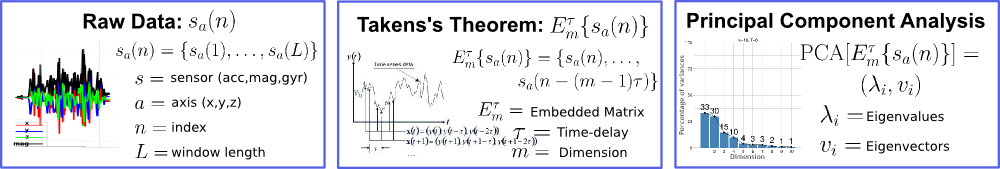
\includegraphics[width=1\textwidth]{method_diagram03}
\caption[PA]{Framework to build the RSS}
 \label{fig:sn}
\end{figure}


\end{frame}
%---------------------------------------------------








%+++++++++++++++++++++++++++++++++++++++++++++++++++
%+++++++++++++++++++++++++++++++++++++++++++++++++++
\section{III. Experiment -- Human-Humanoid Imitation}



%+++++++++++++++++++++++++++++++++++++++++++++++++++
%+++++++++++++++++++++++++++++++++++++++++++++++++++
\subsection{A. Experiment Design}

%+++++++++++++++++++++++++++++++++++++++++++++++++++
\begin{frame}
\frametitle{ Experiment Design }
\vspace{-0.7cm}


\begin{figure}[!htb]
\centering
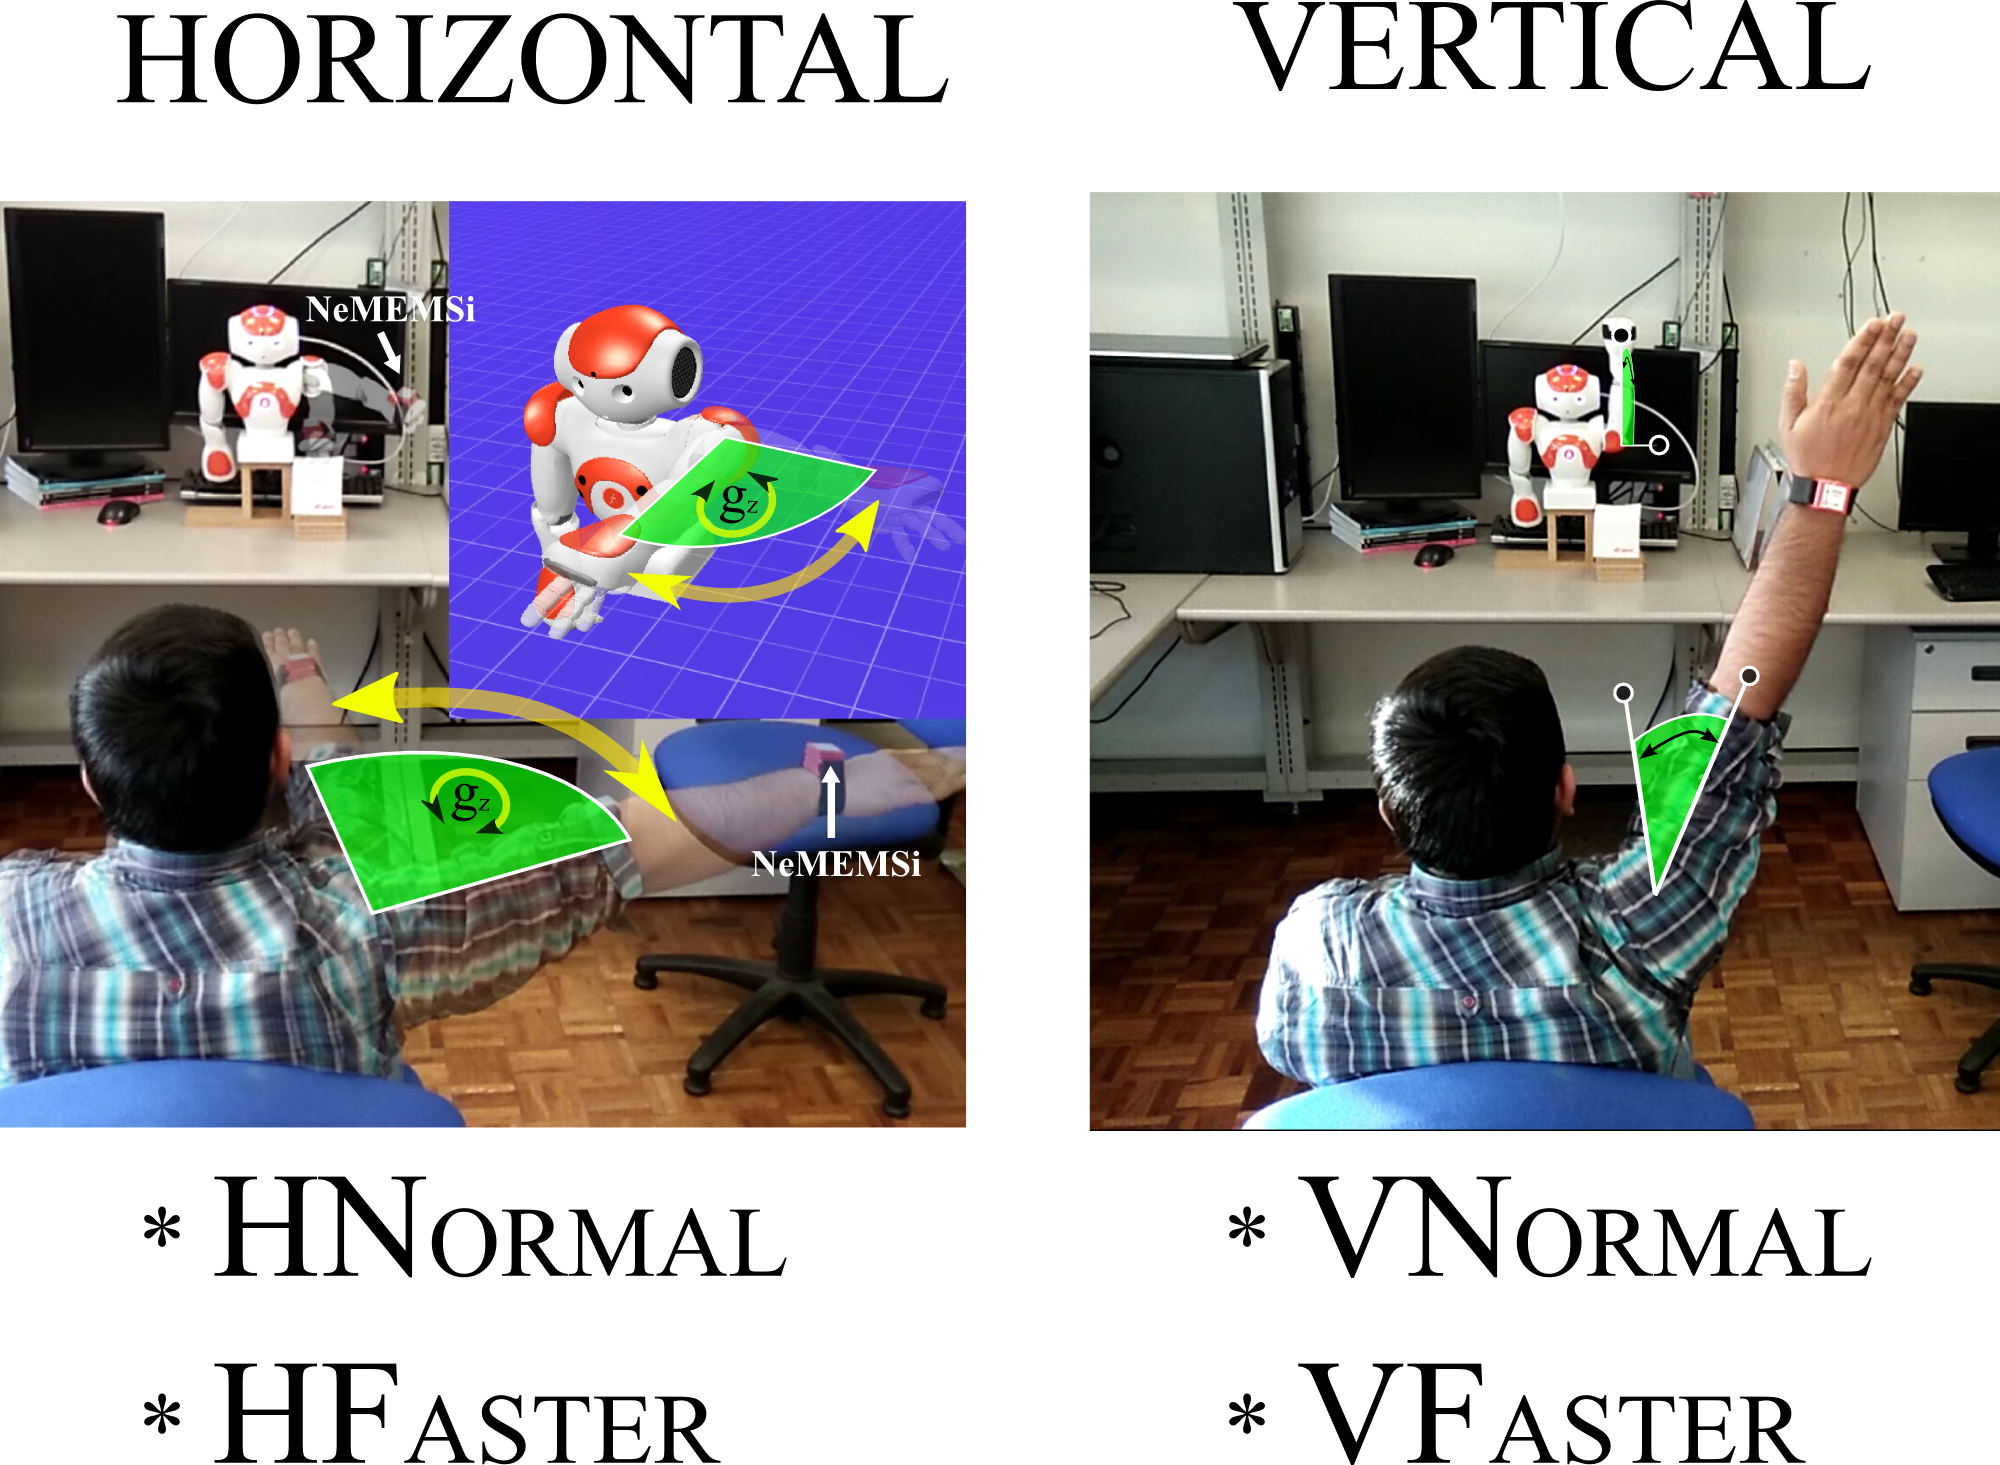
\includegraphics[width=0.75\textwidth]{Xochicale2017Presentation}
\caption[PA]{Front-to-Front Human-Humanoid Imitation Using Wearable Inertial Sensors
}
\label{fig:sn}
\end{figure}

\end{frame}
%---------------------------------------------------





%+++++++++++++++++++++++++++++++++++++++++++++++++++
%+++++++++++++++++++++++++++++++++++++++++++++++++++
\subsection{B. Participants}



%+++++++++++++++++++++++++++++++++++++++++++++++++++
\begin{frame}
\frametitle{Participants}
\vspace{-0.7cm}

Twenty right-handed healthy participants (two females and
ten males) with a mean age of 19.5$\pm$0.79 (from now on ab-
breviated as p01 to p12) were invited to participate in this
study.

% Twenty participants with different years of experience
% in dancing were invited to dance basic salsa steps:
%
% \begin{itemize}
%     \item eleven (4 female, 7 male) novice dancers (none or less than two months of experience);
%     \item one male intermediate (4 years of experience); and,
%     \item one male expert (14 years of experience)
% \end{itemize}



\end{frame}
%---------------------------------------------------







% % \subsection{Design}
%
%
%
%
%
% %+++++++++++++++++++++++++++++++++++++++++++++++++++
% \begin{frame}
% \frametitle{Basic Salsa Steps}
% \vspace{-0.7cm}
%
%
% \begin{figure}[!htb]
% \centering
% 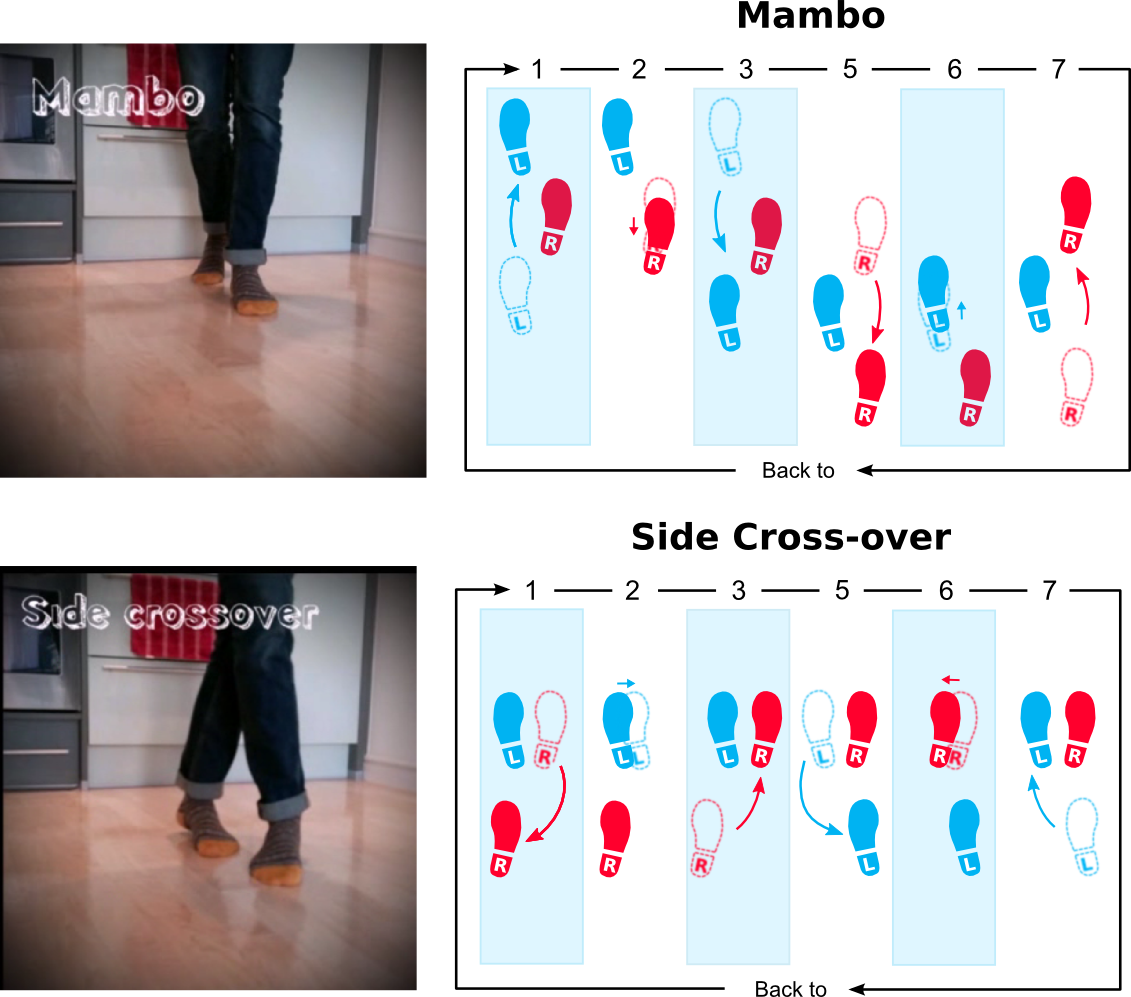
\includegraphics[width=0.7\textwidth]{steps00}
% \caption[PA]{}
%
% \label{fig:sn}
% \end{figure}
%
%
%
% \end{frame}
% %---------------------------------------------------

% %+++++++++++++++++++++++++++++++++++++++++++++++++++
% %+++++++++++++++++++++++++++++++++++++++++++++++++++
% \subsection{E. Data Collection}
%
%
%
%
%
%
%
%
% %+++++++++++++++++++++++++++++++++++++++++++++++++++
% \begin{frame}
% \frametitle{Razor 9DOF IMU}
% \vspace{-0.7cm}
%
% Data collection from Triaxial Accelerometer, gyroscope and magnetometer sensors
% at a sampling rate of 50Hz.
%
% \begin{figure}[!htb]
% \centering
% 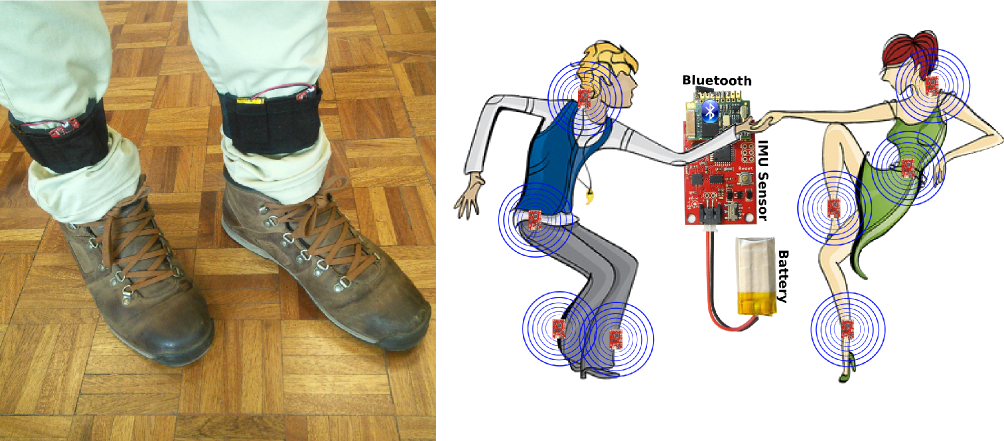
\includegraphics[width=0.7\textwidth]{datacollection01}
% \caption[PA]{IMU sensors mounted on left and right ankle}
%
% \label{fig:sn}
% \end{figure}
%
%
%
% \end{frame}
% %---------------------------------------------------
%
%
%
% %




 %+++++++++++++++++++++++++++++++++++++++++++++++++++
%+++++++++++++++++++++++++++++++++++++++++++++++++++
\section{III. Some Preliminary Results}



\subsection{A. Timeseries of Accelerometer}


%+++++++++++++++++++++++++++++++++++++++++++++++++++
\begin{frame}
\frametitle{Raw Data from the Humanoid}


\begin{adjustwidth}{-3em}{-3em}
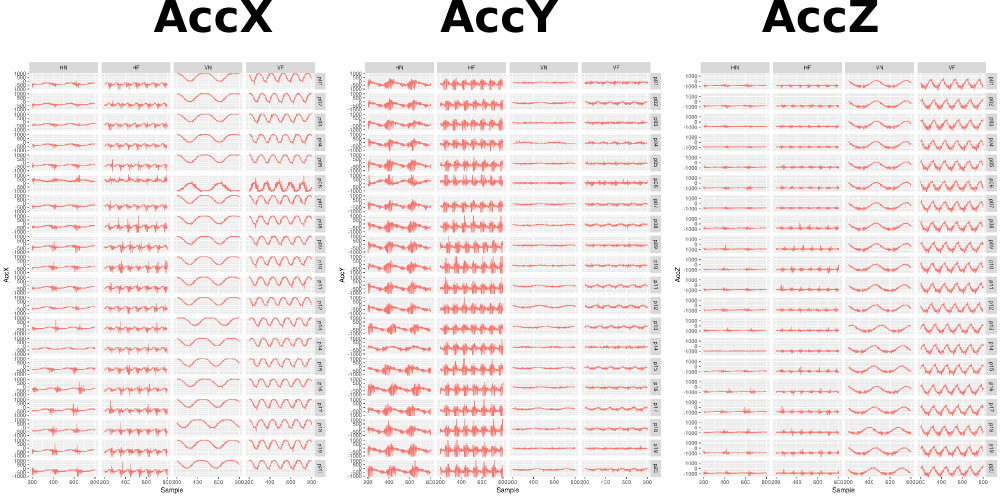
\includegraphics[width=1.2\textwidth]{RS01}
\end{adjustwidth}

\end{frame}
%---------------------------------------------------



%+++++++++++++++++++++++++++++++++++++++++++++++++++
\begin{frame}
\frametitle{Smoothed Data from the Humanoid}


\begin{adjustwidth}{-3em}{-3em}
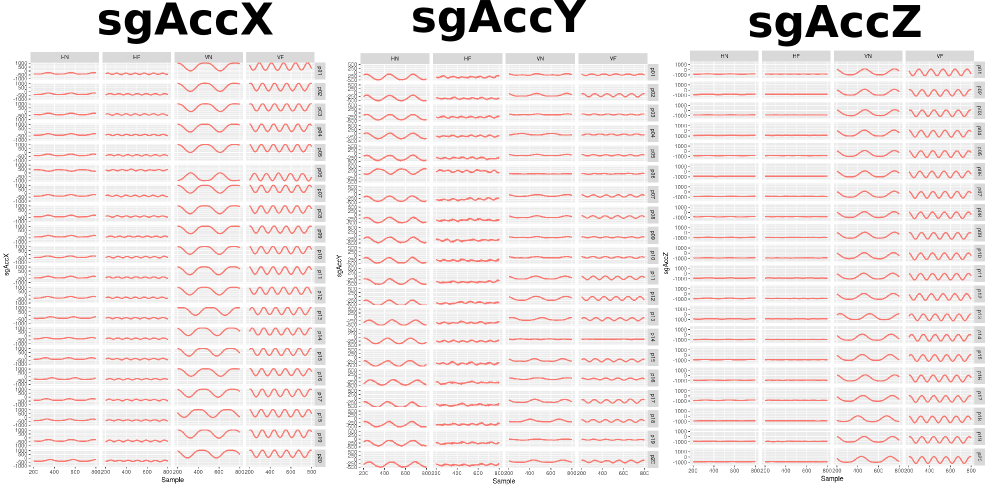
\includegraphics[width=1.2\textwidth]{RsgS01}
\end{adjustwidth}

\end{frame}
%---------------------------------------------------



%+++++++++++++++++++++++++++++++++++++++++++++++++++
\begin{frame}
\frametitle{Raw Data from the Human}


\begin{adjustwidth}{-3em}{-3em}
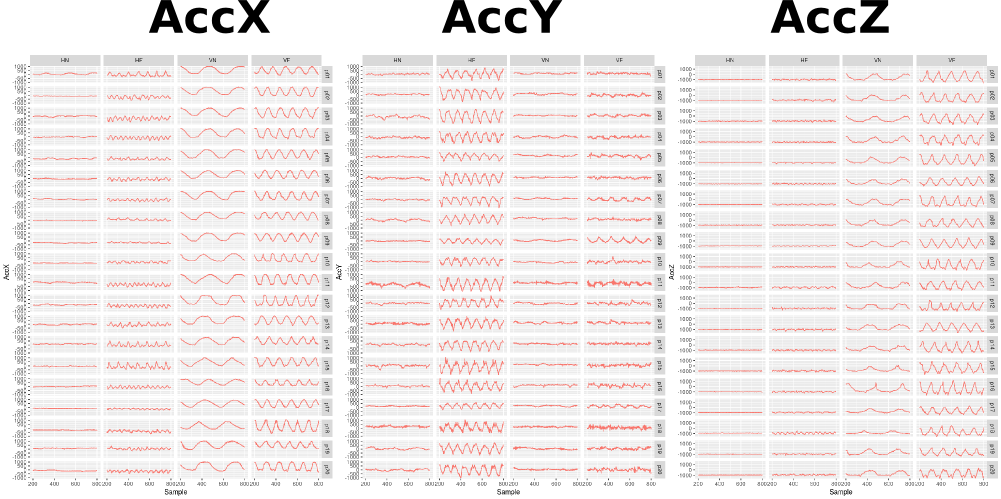
\includegraphics[width=1.2\textwidth]{HS01}
\end{adjustwidth}

\end{frame}
%---------------------------------------------------



%+++++++++++++++++++++++++++++++++++++++++++++++++++
\begin{frame}
\frametitle{Smoothed Data from the Human}


\begin{adjustwidth}{-3em}{-3em}
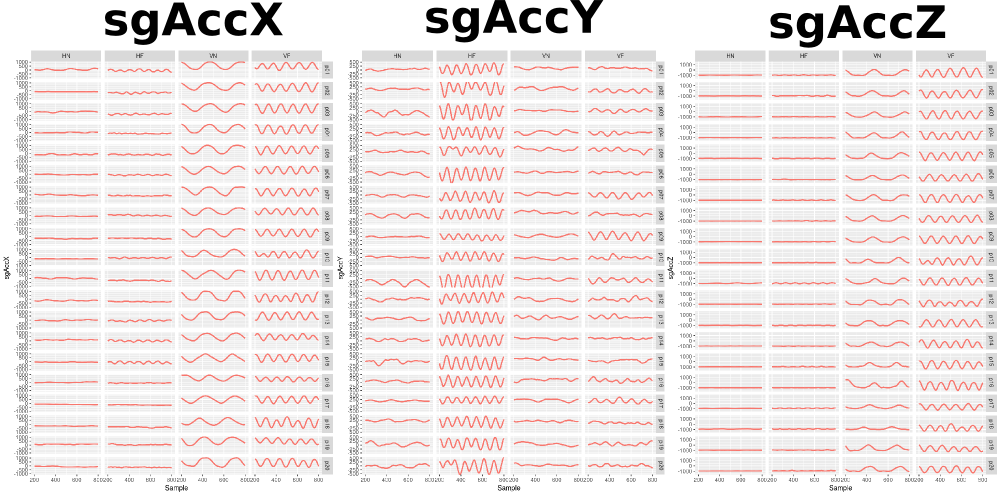
\includegraphics[width=1.2\textwidth]{HsgS01}
\end{adjustwidth}

\end{frame}
%---------------------------------------------------




\subsection{B. Reconstructed State Space }


%+++++++++++++++++++++++++++++++++++++++++++++++++++
\begin{frame}
\frametitle{RSS for Humanoid trial01 sgAccX}

RSS with $m=40$, $\tau=10$
\begin{adjustwidth}{-3em}{-3em}
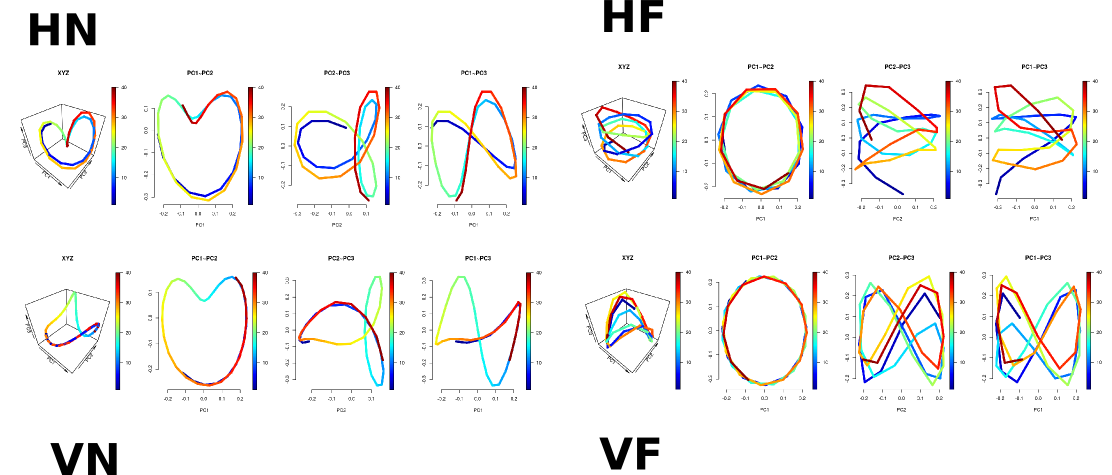
\includegraphics[width=1.2\textwidth]{Robot_p01rss}
\end{adjustwidth}

\end{frame}
%---------------------------------------------------


%+++++++++++++++++++++++++++++++++++++++++++++++++++
\begin{frame}
\frametitle{RSS for Humanoid trial10 sgAccX}

RSS with $m=40$, $\tau=10$
\begin{adjustwidth}{-3em}{-3em}
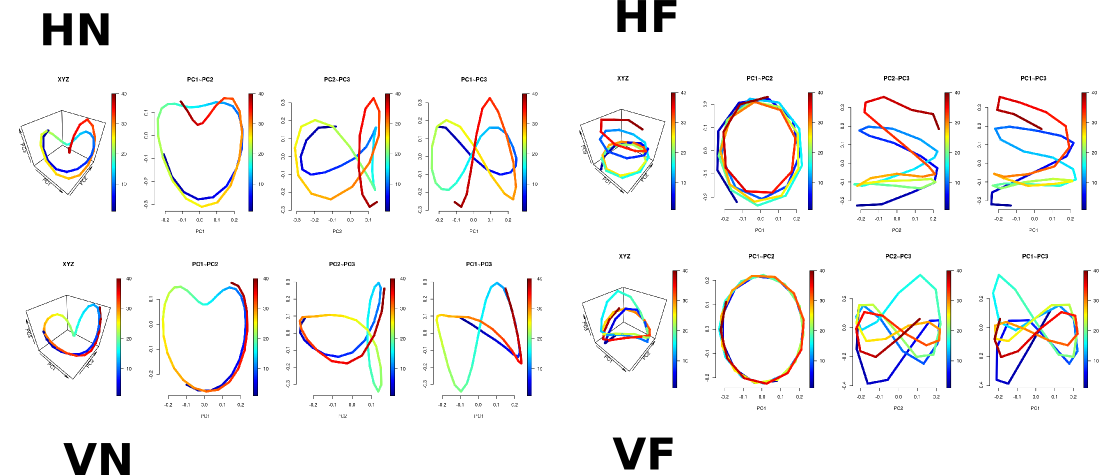
\includegraphics[width=1.2\textwidth]{Robot_p10rss}
\end{adjustwidth}

\end{frame}
%---------------------------------------------------

%+++++++++++++++++++++++++++++++++++++++++++++++++++
\begin{frame}
\frametitle{RSS for Humanoid trial20 sgAccX}

RSS with $m=40$, $\tau=10$
\begin{adjustwidth}{-3em}{-3em}
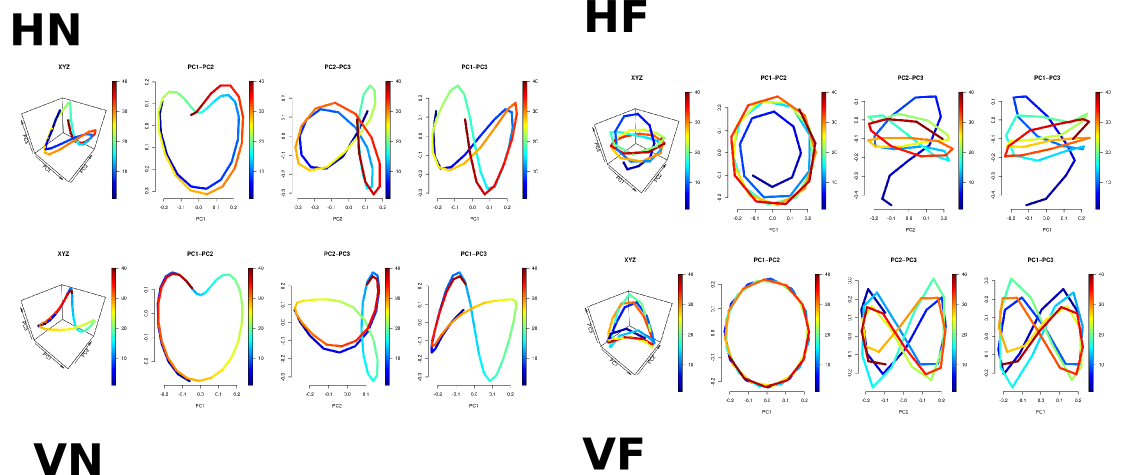
\includegraphics[width=1.2\textwidth]{Robot_p20rss}
\end{adjustwidth}

\end{frame}
%---------------------------------------------------




%+++++++++++++++++++++++++++++++++++++++++++++++++++
\begin{frame}
\frametitle{RSS for Human p01 sgAccX}

RSS with $m=40$, $\tau=10$
\begin{adjustwidth}{-3em}{-3em}
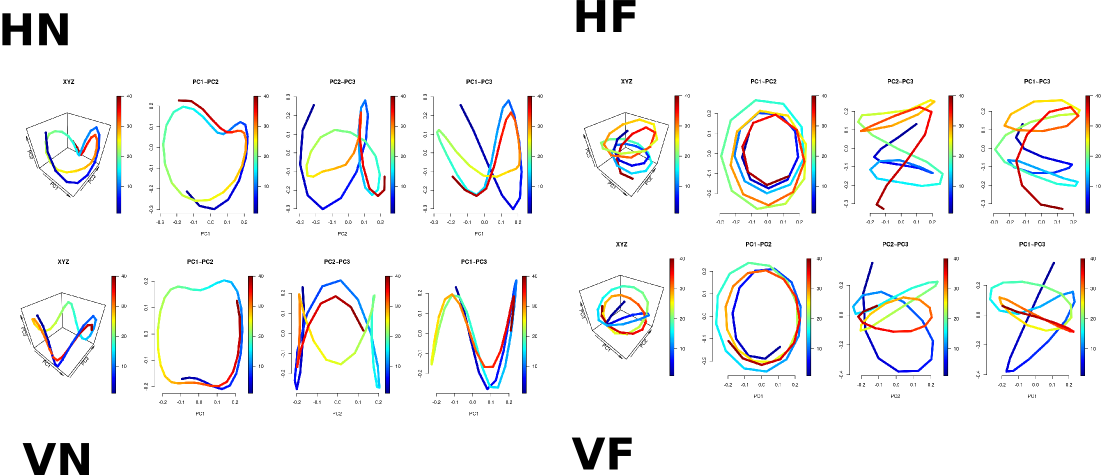
\includegraphics[width=1.2\textwidth]{Humans_p01rss}
\end{adjustwidth}

\end{frame}
%---------------------------------------------------


%+++++++++++++++++++++++++++++++++++++++++++++++++++
\begin{frame}
\frametitle{RSS for Human p10 sgAccX}

RSS with $m=40$, $\tau=10$
\begin{adjustwidth}{-3em}{-3em}
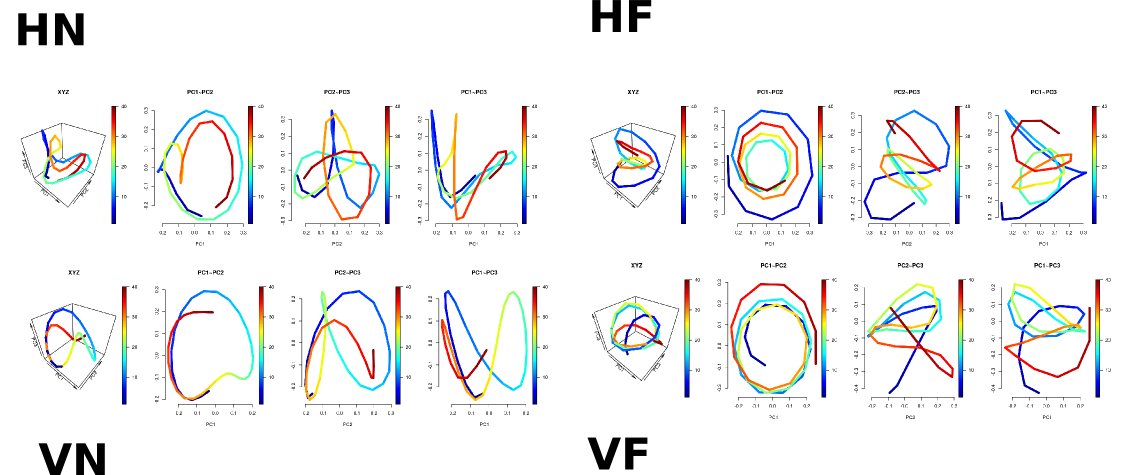
\includegraphics[width=1.2\textwidth]{Humans_p10rss}
\end{adjustwidth}

\end{frame}
%---------------------------------------------------



%+++++++++++++++++++++++++++++++++++++++++++++++++++
\begin{frame}
\frametitle{RSS for Human p20 sgAccX}

RSS with $m=40$, $\tau=10$
\begin{adjustwidth}{-3em}{-3em}
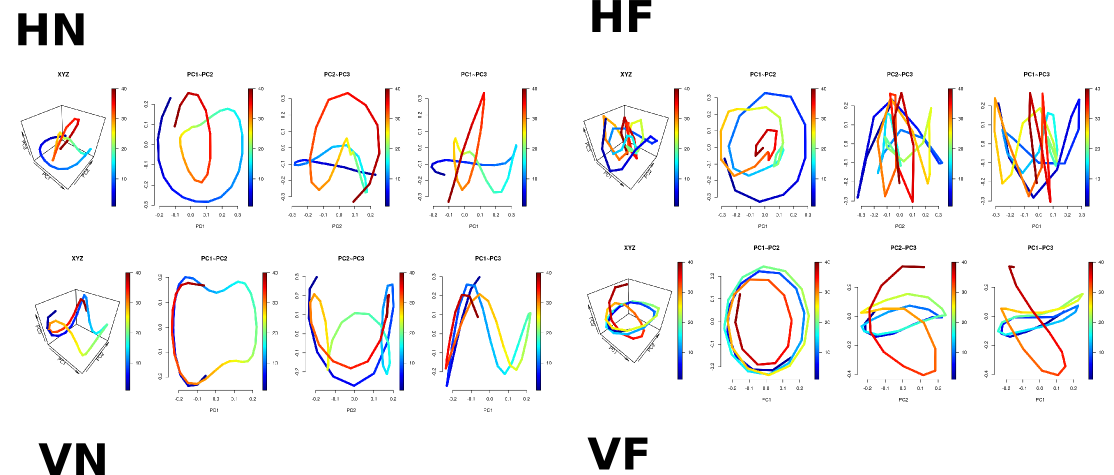
\includegraphics[width=1.2\textwidth]{Humans_p20rss}
\end{adjustwidth}

\end{frame}
%---------------------------------------------------






%+++++++++++++++++++++++++++++++++++++++++++++++++++
\begin{frame}
\frametitle{Euclidean Distances in the RSS}

RSS with $m=40$, $\tau=10$ \\


 \centering
% \begin{adjustwidth}{-3em}{-3em}
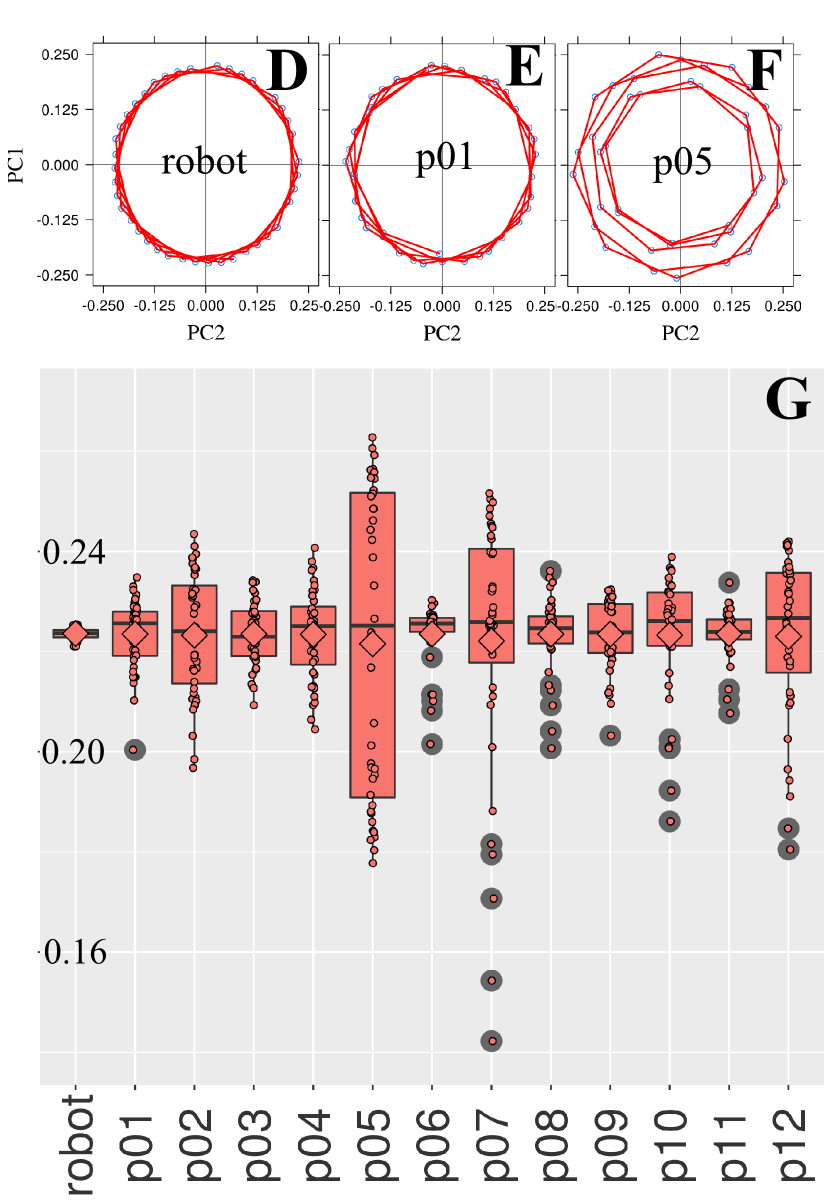
\includegraphics[width=0.4\textwidth]{Xochicale2017Fig1b}
% \end{adjustwidth}

\end{frame}
%---------------------------------------------------




%+++++++++++++++++++++++++++++++++++++++++++++++++++
%+++++++++++++++++++++++++++++++++++++++++++++++++++
\section{IV. Conclusions and Future Work}









%+++++++++++++++++++++++++++++++++++++++++++++++++++
\begin{frame}
\frametitle{Conclusions and Future Work}
\vspace{-0.7cm}

Pros and Cons of RSS
    \begin{itemize}
    \item (+) The RSS provide a visually a good representation of the variability of the
    activities.
    \item (-) The quality of the Euclidean distances in the RSS
    is debatable and needs further investigation.
    \end{itemize}

TODO List:
\begin{itemize}
    \item Have better understanding of the time-delay embedding theorem
    \item Implement the Lyapunov Exponent.
    \item Use Convolutional Neural Networks to classify Movement Variability
    \end{itemize}

\end{frame}
%---------------------------------------------------


%+++++++++++++++++++++++++++++++++++++++++++++++++++
\begin{frame}
\frametitle{}

\vspace{2cm}
\begin{center}
\LARGE{QUESTIONS?}
\end{center}

\vspace{1cm}

\normalsize
\textbf{Miguel P. Xochicale} \\
Doctoral Researcher in Human-Robot Interaction (2014-2018)\\
University of Birmingham, U.K. \\
{\color{blue} \href{http://mxochicale.github.io/}{http://mxochicale.github.io/ } } \\


\vspace{1cm}



\includegraphics[scale=.4]{CC4}
\tiny{
\textbf{My own pictures are release under CC BY-NC 4.0
{\color{blue} \href{http://creativecommons.org/licenses/by-nc/4.0/}{http://creativecommons.org/licenses/by-nc/4.0/} } \\
Give credits to: Miguel P. Xochicale
}
}

\end{frame}
%---------------------------------------------------




%   \section[allowframebreaks]{References}

%  \section{V. Conclusions and Future Work}


 \begin{frame}[fragile,allowframebreaks]{References}
  % In your presentation, remove `\nocite` here and
  % use `\cite` throughout the presentation.
  \nocite{*}

  \bibliographystyle{apalike}
  \bibliography{refslides}


%  \bibliography{D:/Gpai/Biblographies/library}
\end{frame}






%
% % Creates the cover page.
%  \frame{\titlepage}



\end{document}
